% !TEX root = template.tex

\section{Simulation framework}
\label{sec:simulation_framework}
% The aim of this paper is to compare the behavior of three different communication technologies within a similar scenario. 
To compare different communication technologies, the authors developed three independent scenarios using WAVE, LENA and mmwave module for \textit{ns-3}. The latter is not in the official release but has been developed by University of Padua toghether with New York University (NYU) as an extension of LENA module to allow realistic simulations also for higher frequency applications. 

The simulation's scenario is slight different for \gls{dsrc} and the other two technologies. In a realistic scenario, \gls{dsrc} is used mostly in direct \gls{v2v} communication, LTE is more suitable for a \gls{v2i} communication and \gls{mmWaves} can be used both in a \gls{v2v} communication (assuming the vehicles are in line of sight and close to each other and assuming good enough environment conditions) and a \gls{v2i} one.
Nevertheless, in this paper \gls{mmWaves} is considered only for \gls{v2i} communication.

\subsection{DSRC}
\label{sec:dsrc_model}
To simulate the robustness and the feasibility of \gls{dsrc} in our application, two vehicles have been positioned in \gls{los}, they do not move during the simulation and their distance is increased from a minimum of 2 meters to a maximum of 200 meters. This scenario takes into account both the case in which the cars are actually stopped and when, instead, the cars are moving with the same velocity and the same direction.

A vehicle sends to the other 1000 bytes packets using UDP and 3 different inter-packet intervals: $8\mu s$, $80\mu s$ and $0.8s$, that correspond respectively to the datarates: $1Gb/s$, $100Mb/s$ and $10kb/s$.

The simulation has been made using the \gls{wave} module of ns-3 that implements the core features of \gls{dsrc} standards suite \cite{WAVEStandard}.

\subsection{LTE}
LTE is the most used technology in the $4^{th}$ generation cellular networks, therefore is used as backup technology in case \gls{dsrc} or \gls{mmWaves} are not usable due to environment conditions, the requirements of the application to use or any other reason.

The scenario implemented to simulate the behavior of LTE is a square area 500 meters wide in which 6 buildings and \gls{enodeb} (i.e. the LTE base stations in 3GPP \gls{nr} terminology) are randomly positioned.
The number of \gls{enodeb}s positioned in the area increases from 3 to 40. This high density of base stations is irrealistic for LTE, since each \gls{enodeb} can give a coverage up to several km, but is used anyway to have data comparable with \gls{mmWaves}' simulations.
User moves from (100, 490) as shown in \fig{fig:scenario}, with a velocity of $30m/s$ for 10 seconds. During the simulation, it receives 1400 bytes packets from the closest eNodeB at a rate of $1.12 Gb/s$ and $50Mb/s$.

Handovers are made from an eNodeB to another, if needed, in order to receive the best signal in each moment. \textit{LENA} module of ns-3 has been used for the simulation.

\begin{figure}[ht]
\vspace{-0.2in}
  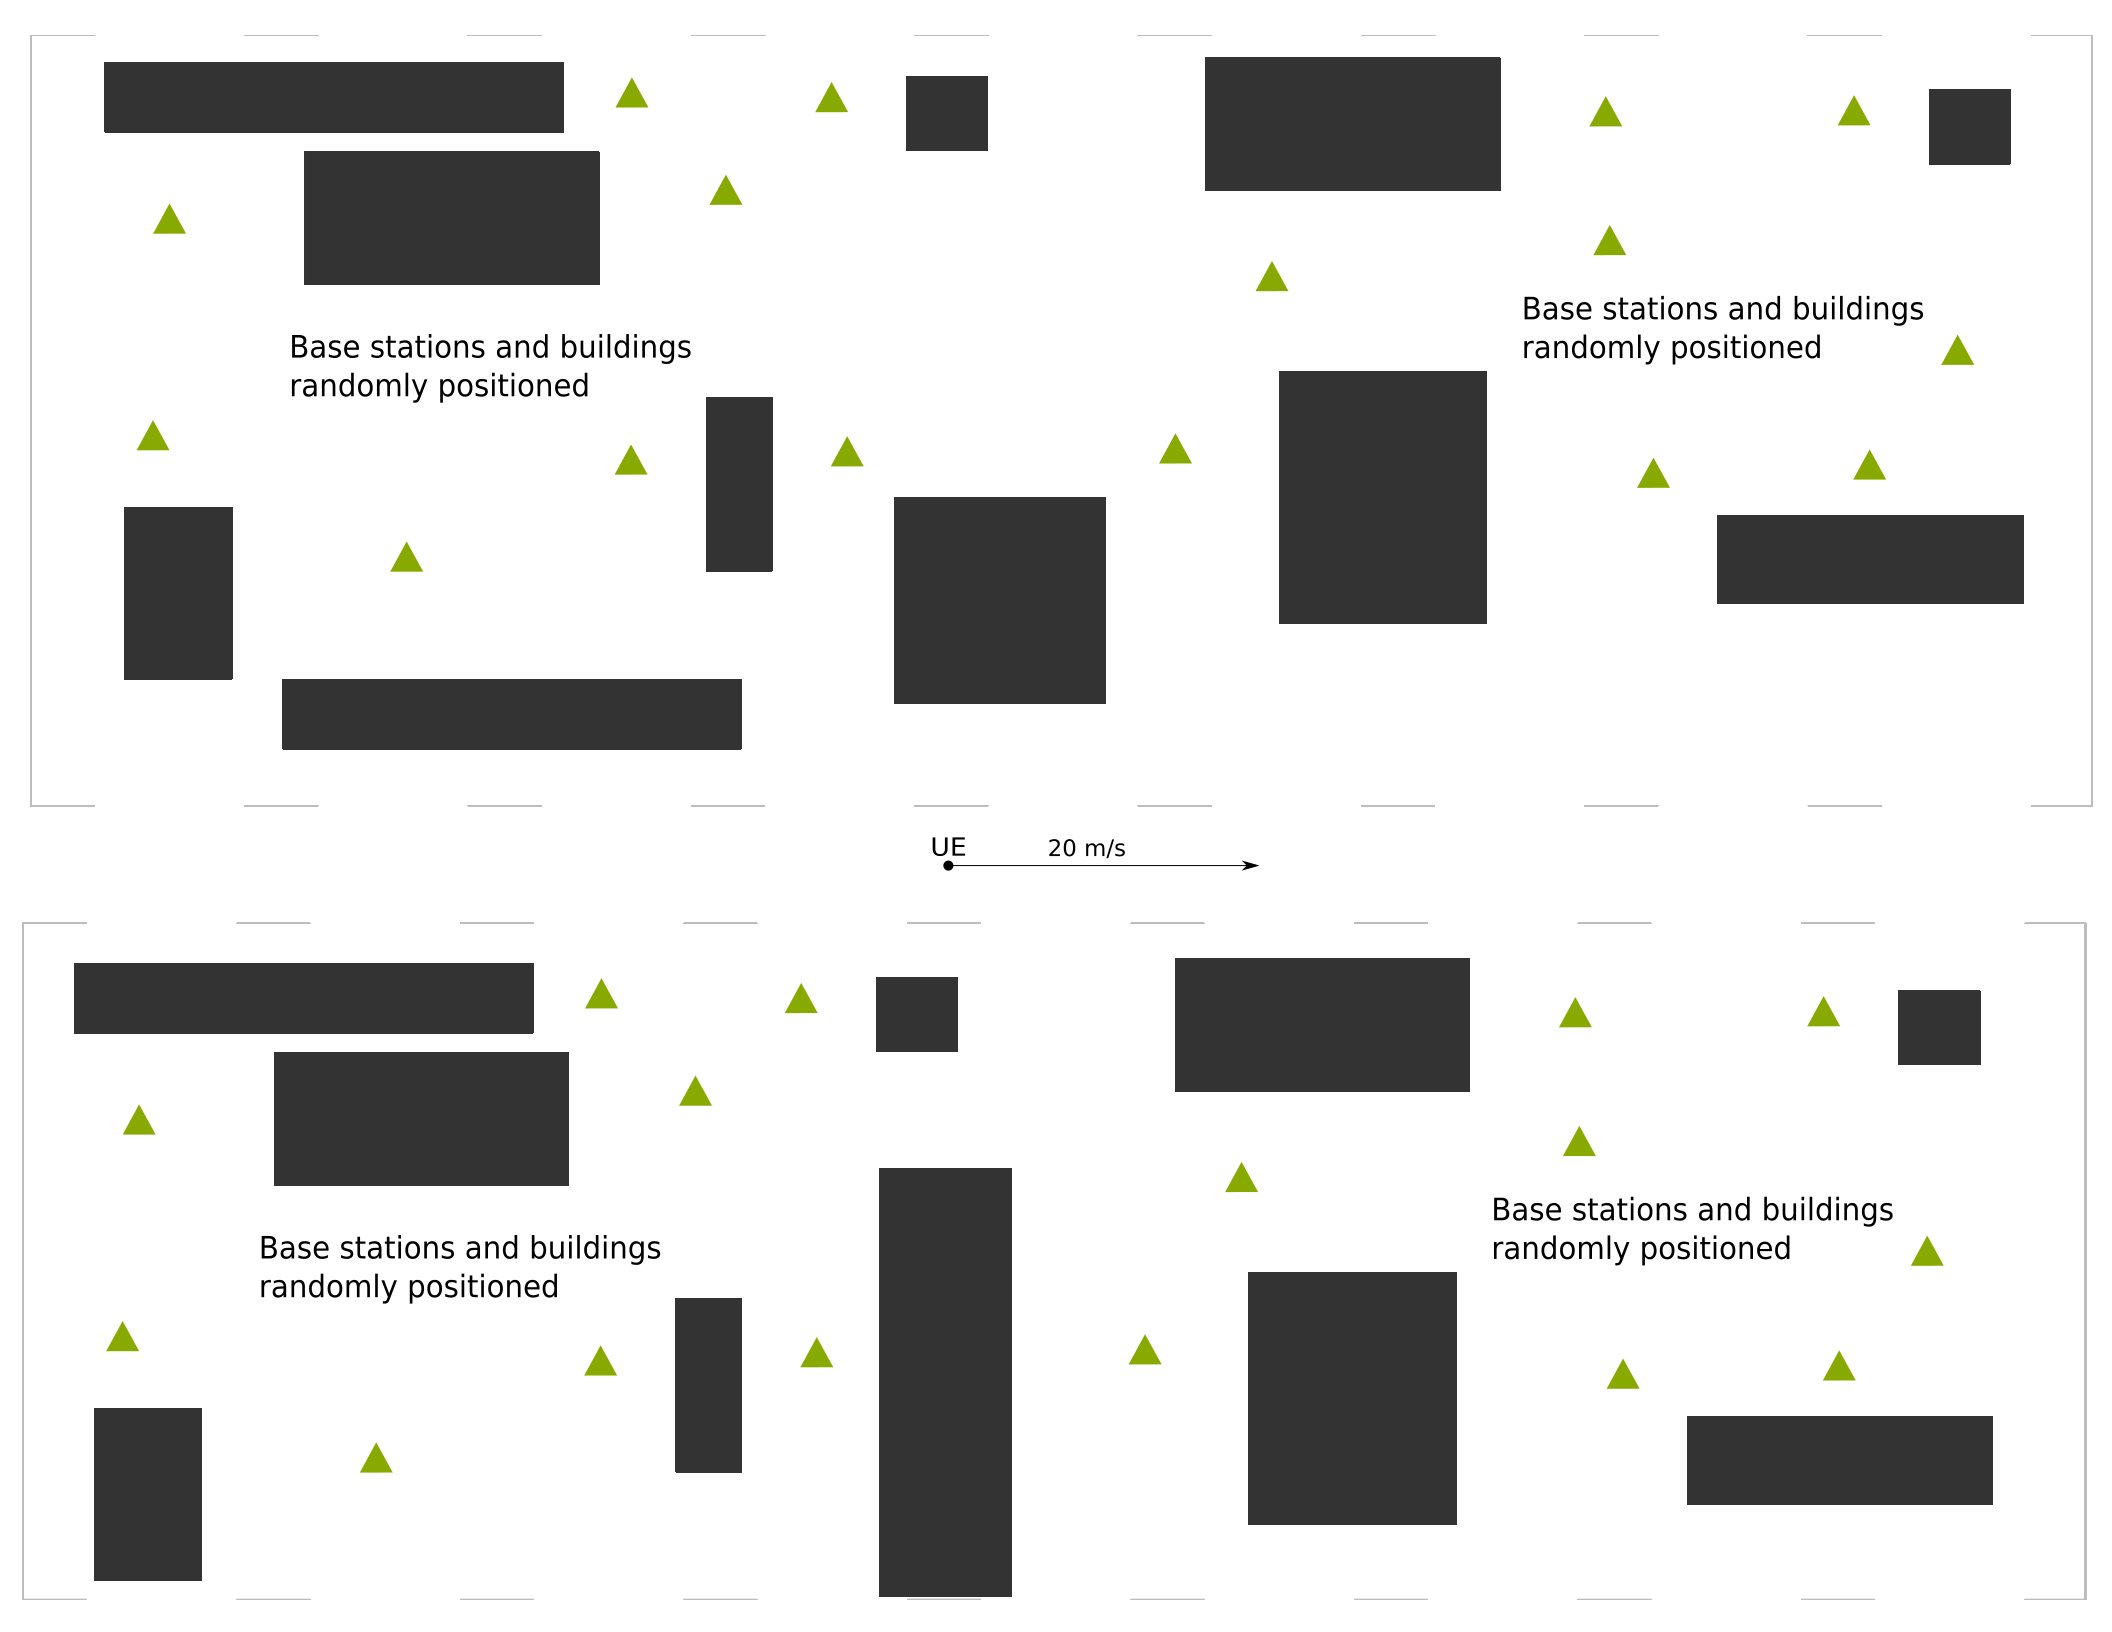
\includegraphics[width=\linewidth]{scenario}
  \caption{Example of a simulation scenario, \gls{enodeb}s and buildings are generated randomly in the designated area.}
  \label{fig:scenario}
\end{figure}

\subsection{mmWaves}
The solution adopted to simulate \gls{mmWaves} is the same used for LTE, this time 40 \gls{gnb} (i.e. the mmWaves base stations in 3GPP \gls{nr} terminology) in a square area 500 meters wide is a realistic scenario since each \gls{gnb} has a very small coverage area due to the blockage problem of high frequency technologies.

For this part, an ns-3 module implemented by University of Padua and NYU has been used \cite{Mezzavilla18}, that implements the PHY and MAC layer of mmWaves in a modular and higly customizable manner.